\section{Consuntivo}
Di seguito si analizza lo scostamento tra le spese effettive per ogni ruolo e il preventivo. Tra parentesi viene indicato:
\begin{itemize}
	\item $-numero$: se sono state utilizzate meno ore / soldi di quelli preventivati;
	\item $+0$: se sono state utilizzate tutte e sole le ore / soldi preventivati;
	\item $+numero$: se sono state utilizzate più ore / soldi di quelli preventivati.
\end{itemize}
\subsection{Periodo di Analisi}
Le ore impiegate per il periodo di analisi sono considerate come ore di investimento personale per cui non sono rendicontate.
\begin{table}[H]
	\rowcolors{2}{lightest-grayest}{white}
	\centering
	\renewcommand{\arraystretch}{1.5}
	\begin{tabular}{|c|c|c|}
		\hline
		\rowcolor{lighter-grayer}
Ruolo & Ore & Costo \\ \hline
Responsabile & 34(+0) & 1020(+0\euro) \\ \hline
Amministratore & 64(+3) & 1408(+66\euro) \\ \hline
Analista & 79(+6) & 1975(+150\euro) \\ \hline
Progettista & 0(+0) & 0(+0\euro) \\ \hline
Programmatore & 0(+0) & 0(+0\euro) \\ \hline
Verificatore & 82(+3) & 1312(+48\euro) \\ \hline
Totale preventivo & 259 & 5715\euro \\ \hline
Totale consuntivo & 271 & 5979\euro \\ \hline
Totale scostamento & +12 & +264\euro \\ \hline
	\end{tabular}
	\caption*{\textbf{Tabella 21}: Consuntivo riguardante il periodo di Analisi\\}
\end{table}
\subsubsection{Conclusioni}
Come emerge dalla tabella precedente è stato necessario investire più tempo di quanto preventivato
nei ruoli di Amministratore, Analista e Verificatore.
Il bilancio risultante è negativo e di seguito sono esposte le cause dei ritardi:
\begin{itemize}
	\item Amministratore: è stato necessario più tempo del previsto per individuare uno scheletro per la stesura del Piano di Qualifica. In particolare,
	nella ricerca della modalità per parallelizzare i compiti il più possibile, senza perdere in termini di uniformità del documento;
	\item Analista: alcuni requisiti si sono rivelati di non facile comprensione, quindi sono state necessarie 
	più ore di lavoro del previsto;
	\item Verificatori: alcuni requisiti sono stati individuati tardivamente e di conseguenza per
	l’aggiunta di contenuti nel documento di Analisi dei Requisiti è stato necessario impiegare
	qualche ora in più per controllare nuovamente il documento.
\end{itemize}
\subsubsection{Preventivo a finire}
Il preventivo a finire presenta un surplus di 264\euro, poiché in questo periodo di analisi sono state necessarie più ore del previsto.
Ciò non è ritenuto un problema in quanto le ore lavorative e i costi sostenuti in questo periodo non verranno rendicontati.

\subsection{Periodo di Progettazione Architetturale (dal 2021-01-18 al 2021-03-07) }
\subsubsection{Consuntivo di macroperiodo}

\begin{table}[H]
	\centering
	\begin{tabular}{|l|l|l|l|l|l|l|}
		\hline
		\rowcolor{lighter-grayer}
		\textbf{Attività}            & \textbf{Re}         & \textbf{Am}         & \textbf{An}         & \textbf{Pt}        & \textbf{Pm}        & \textbf{Ve}         \\ \hline
		Aggiornamento PdQ            & \multirow{4}{*}{10} & \multirow{4}{*}{10} & \multirow{4}{*}{20} & \multirow{4}{*}{-} & \multirow{4}{*}{-} & \multirow{4}{*}{15} \\ \cline{1-1}
		Aggiornamento AdR            &                     &                     &                     &                    &                    &                     \\ \cline{1-1}
		Aggiornamento NdP            &                     &                     &                     &                    &                    &                     \\ \cline{1-1}
		Aggiornamento PdP            &                     &                     &                     &                    &                    &                     \\ \hline
		Technology baseline          & -                   & -                   & -                   & 20                 & -                  & -                   \\ \hline
		Proof of concept             & -                   & -                   & -                   & 36                 & -                  & -                   \\ \hline
		Attività accessorie          & 2                   & 5                   & 1                   & 2                  & -                  & 4                   \\ \hline
		Comunicazione con docenti    & 1                   & -                   & -                   & -                  & -                  & -                   \\ \hline
		Comunicazione con proponente & -                   & -                   & -                   & -                  & -                  & -                   \\ \hline
		Presentazione                & 1                   & 1                   & 1                   & 1                  & -                  & 1                   \\ \hline
		Attività impreviste          & 1                   & 2                   & -                   & -                  & -                  & -                   \\ \hline
	\end{tabular}
	\caption*{\textbf{Tabella 22}: Prospetto orario reale\\}
\end{table}

\begin{table}[H]
	\rowcolors{2}{lightest-grayest}{white}
	\centering
	\renewcommand{\arraystretch}{1.5}
	\begin{tabular}{|c|c|c|}
		\hline
		\rowcolor{lighter-grayer}
		Ruolo & Ore & Costo \\ \hline
		Responsabile & 15(-6) & 450(-180\euro) \\ \hline
		Amministratore & 18(+6) & 396(132\euro) \\ \hline
		Analista & 22(-20) & 550(-500\euro) \\ \hline
		Progettista & 59(-4) & 1416(-96)\euro \\ \hline
		Programmatore & - & - \\ \hline
		Verificatore & 20(-11) & 320(-176\euro) \\ \hline
		Totale preventivo & 169 & 3952\euro \\ \hline
		Totale consuntivo & 134 & 3132\euro \\ \hline
		Totale scostamento & -35 & -820\euro \\ \hline
	\end{tabular}
	\caption*{\textbf{Tabella 23}: Consuntivo\\}
\end{table}
\begin{figure}[H]
	\centering
	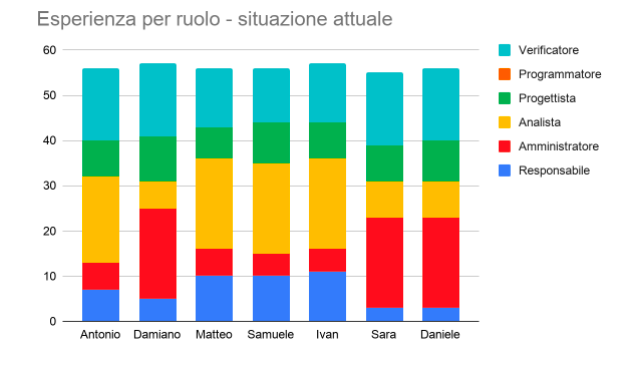
\includegraphics[width=15cm]{res/images/GraficoRuoli.png}
	\caption*{\textbf{Figura 15}: Esperienza per ruolo}
	\label{fig:Esperienza per ruolo}
\end{figure}

\subsubsection{Consuntivo di microperiodo}
\paragraph{Microperiodo 1}
\begin{table}[H]
	\centering
	\begin{tabular}{|c|c|c|c|c|c|c|}
		\hline
		\rowcolor{lighter-grayer}
		\textbf{Attività} & \textbf{Re}        & \textbf{Am}        & \textbf{An}        & \textbf{Pt}        & \textbf{Pm}        & \textbf{Ve}        \\ \hline
		Aggiornamento PdQ & \multirow{4}{*}{2} & \multirow{4}{*}{2} & \multirow{4}{*}{4} & \multirow{4}{*}{-} & \multirow{4}{*}{-} & \multirow{4}{*}{3} \\ \cline{1-1}
		Aggiornamento AdR &                    &                    &                    &                    &                    &                    \\ \cline{1-1}
		Aggiornamento NdP &                    &                    &                    &                    &                    &                    \\ \cline{1-1}
		Aggiornamento PdP &                    &                    &                    &                    &                    &                    \\ \hline
	\end{tabular}
	\caption*{\textbf{Tabella 24}: Prospetto orario reale\\}
\end{table}

\begin{table}[H]
	\rowcolors{2}{lightest-grayest}{white}
	\centering
	\renewcommand{\arraystretch}{1.5}
	\begin{tabular}{|c|c|c|}
		\hline
		\rowcolor{lighter-grayer}
		Ruolo & Ore & Costo \\ \hline
		Responsabile & 2(+0) & 60(+0\euro) \\ \hline
		Amministratore & 2(+1) & 44(+22\euro) \\ \hline
		Analista & 4(-4) & 100(-100\euro) \\ \hline
		Progettista & - & - \\ \hline
		Programmatore & - & - \\ \hline
		Verificatore & 3(-2) & 48(-32\euro) \\ \hline
		Totale preventivo & 16 & 362\euro \\ \hline
		Totale consuntivo & 11 & 252\euro \\ \hline
		Totale scostamento & 5 & -110\euro \\ \hline
	\end{tabular}
	\caption*{\textbf{Tabella 25}: Consuntivo\\}
\end{table}

\paragraph{Microperiodo 2}
\begin{table}[H]
	\centering
	\begin{tabular}{|c|c|c|c|c|c|c|}
		\hline
		\rowcolor{lighter-grayer}
		\textbf{Attività}                         & \textbf{Re}            & \textbf{Am}            & \textbf{An}            & \textbf{Pt}             & \textbf{Pm}            & \textbf{Ve}            \\ \hline
		Aggiornamento PdQ                         & \multirow{4}{*}{2}     & \multirow{4}{*}{2}     & \multirow{4}{*}{4}     & \multirow{4}{*}{-}      & \multirow{4}{*}{-}     & \multirow{4}{*}{3}     \\ \cline{1-1}
		Aggiornamento AdR                         &                        &                        &                        &                         &                        &                        \\ \cline{1-1}
		Aggiornamento NdP                         &                        &                        &                        &                         &                        &                        \\ \cline{1-1}
		Aggiornamento PdP                         &                        &                        &                        &                         &                        &                        \\ \hline
		\multicolumn{1}{|l|}{Technology baseline} & \multicolumn{1}{l|}{-} & \multicolumn{1}{l|}{-} & \multicolumn{1}{l|}{-} & \multicolumn{1}{l|}{20} & \multicolumn{1}{l|}{-} & \multicolumn{1}{l|}{-} \\ \hline
	\end{tabular}
\caption*{\textbf{Tabella 26}: Prospetto orario reale\\}
\end{table}

\begin{table}[H]
	\rowcolors{2}{lightest-grayest}{white}
	\centering
	\renewcommand{\arraystretch}{1.5}
	\begin{tabular}{|c|c|c|}
		\hline
		\rowcolor{lighter-grayer}
		Ruolo & Ore & Costo \\ \hline
		Responsabile & 2(+0) & 60(+0\euro) \\ \hline
		Amministratore & 2(+1) & 44(+22\euro) \\ \hline
		Analista & 4(+4) & 100(-100\euro) \\ \hline
		Progettista & 20(+0) & 480(+0\euro) \\ \hline
		Programmatore & - & - \\ \hline
		Verificatore & 3(-2) & 48(-32\euro) \\ \hline
		Totale preventivo & 36 & 842\euro \\ \hline
		Totale consuntivo & 31 & 732\euro \\ \hline
		Totale scostamento & -5 & -110\euro \\ \hline
	\end{tabular}
	\caption*{\textbf{Tabella 27}: Consuntivo\\}
\end{table}

\paragraph{Microperiodo 3}
\begin{table}[H]
	\centering
	\begin{tabular}{|c|c|c|c|c|c|c|}
		\hline
		\rowcolor{lighter-grayer}
		\textbf{Attività}     & \textbf{Re}        & \textbf{Am}        & \textbf{An}        & \textbf{Pt}        & \textbf{Pm}        & \textbf{Ve}        \\ \hline
		Aggiornamento PdQ     & \multirow{4}{*}{2} & \multirow{4}{*}{2} & \multirow{4}{*}{4} & \multirow{4}{*}{-} & \multirow{4}{*}{-} & \multirow{4}{*}{3} \\ \cline{1-1}
		Aggiornamento AdR     &                    &                    &                    &                    &                    &                    \\ \cline{1-1}
		Aggiornamento NdP     &                    &                    &                    &                    &                    &                    \\ \cline{1-1}
		Aggiornamento PdP     &                    &                    &                    &                    &                    &                    \\ \hline
		Proof of Concept                   & -                  & -                  & -                  & 20                 & -                  & -                  \\ \hline
		Comunicazioni docenti & 1                  & -                  & -                  & -                  & -                  & -                  \\ \hline
	\end{tabular}
\caption*{\textbf{Tabella 28}: Prospetto orario reale\\}
\end{table}

\begin{table}[H]
	\rowcolors{2}{lightest-grayest}{white}
	\centering
	\renewcommand{\arraystretch}{1.5}
	\begin{tabular}{|c|c|c|}
		\hline
		\rowcolor{lighter-grayer}
		Ruolo & Ore & Costo \\ \hline
		Responsabile & 3(+0) & 90(+0\euro) \\ \hline
		Amministratore & 2(+1) & 44(+22\euro) \\ \hline
		Analista & 4(+4) & 100(-100\euro) \\ \hline
		Progettista & 20(+0) & 480(+0\euro) \\ \hline
		Programmatore & - & - \\ \hline
		Verificatore & 3(-2) & 48(-32\euro) \\ \hline
		Totale preventivo & 37 & 872\euro \\ \hline
		Totale consuntivo & 32 & 762\euro \\ \hline
		Totale scostamento & -5 & -110\euro \\ \hline
	\end{tabular}
	\caption*{\textbf{Tabella 29}: Consuntivo\\}
\end{table}

\paragraph{Microperiodo 4}
\begin{table}[H]
	\centering
	\begin{tabular}{|c|c|c|c|c|c|c|}
		\hline
		\rowcolor{lighter-grayer}
		\textbf{Attività} & \textbf{Re}        & \textbf{Am}        & \textbf{An}        & \textbf{Pt}        & \textbf{Pm}        & \textbf{Ve}        \\ \hline
		Aggiornamento PdQ & \multirow{4}{*}{2} & \multirow{4}{*}{2} & \multirow{4}{*}{4} & \multirow{4}{*}{-} & \multirow{4}{*}{-} & \multirow{4}{*}{3} \\ \cline{1-1}
		Aggiornamento AdR &                    &                    &                    &                    &                    &                    \\ \cline{1-1}
		Aggiornamento NdP &                    &                    &                    &                    &                    &                    \\ \cline{1-1}
		Aggiornamento PdP &                    &                    &                    &                    &                    &                    \\ \hline
		Proof of Concept               & -                  & -                  & -                  & 16                 & -                  & -                  \\ \hline
	\end{tabular}
\caption*{\textbf{Tabella 30}: Prospetto orario reale\\}
\end{table}

\begin{table}[H]
	\rowcolors{2}{lightest-grayest}{white}
	\centering
	\renewcommand{\arraystretch}{1.5}
	\begin{tabular}{|c|c|c|}
		\hline
		\rowcolor{lighter-grayer}
		Ruolo & Ore & Costo \\ \hline
		Responsabile & 2(-1) & 60(-30\euro) \\ \hline
		Amministratore & 2(+1) & 44(+22\euro) \\ \hline
		Analista & 4(+4) & 100(-100\euro) \\ \hline
		Progettista & 16(-4) & 384(-96\euro) \\ \hline
		Programmatore & - & - \\ \hline
		Verificatore & 3(-2) & 48(-32\euro) \\ \hline
		Totale preventivo & 37 & 872\euro \\ \hline
		Totale consuntivo & 27 & 636\euro \\ \hline
		Totale scostamento & -10 & -236\euro \\ \hline
	\end{tabular}
	\caption*{\textbf{Tabella 31}: Consuntivo\\}
\end{table}

\paragraph{Microperiodo 5}
\begin{table}[H]
	\centering
	\begin{tabular}{|c|c|c|c|c|c|c|}
		\hline
		\rowcolor{lighter-grayer}
		\textbf{Attività}   & \textbf{Re}        & \textbf{Am}        & \textbf{An}        & \textbf{Pt}        & \textbf{Pm}        & \textbf{Ve}        \\ \hline
		Aggiornamento PdQ   & \multirow{4}{*}{2} & \multirow{4}{*}{2} & \multirow{4}{*}{4} & \multirow{4}{*}{-} & \multirow{4}{*}{-} & \multirow{4}{*}{3} \\ \cline{1-1}
		Aggiornamento AdR   &                    &                    &                    &                    &                    &                    \\ \cline{1-1}
		Aggiornamento NdP   &                    &                    &                    &                    &                    &                    \\ \cline{1-1}
		Aggiornamento PdP   &                    &                    &                    &                    &                    &                    \\ \hline
		Presentazione       & 1                  & 1                  & 1                  & 1                  & -                  & 1                  \\ \hline
		Attività accessorie & 2                  & 5                  & 1                  & 2                  & -                  & 4                  \\ \hline
		Attività impreviste & 1                  & 2                  & -                  & -                  & -                  & -                  \\ \hline
	\end{tabular}
\caption*{\textbf{Tabella 32}: Prospetto orario reale\\}
\end{table}

\begin{table}[H]
	\rowcolors{2}{lightest-grayest}{white}
	\centering
	\renewcommand{\arraystretch}{1.5}
	\begin{tabular}{|c|c|c|}
		\hline
		\rowcolor{lighter-grayer}
		Ruolo & Ore & Costo \\ \hline
		Responsabile & 6(+0) & 180(+0\euro) \\ \hline
		Amministratore & 10(+2) & 220(+44\euro) \\ \hline
		Analista & 6(-4) & 150(-100\euro) \\ \hline
		Progettista & 3(+0) & 72(+0\euro) \\ \hline
		Programmatore & - & - \\ \hline
		Verificatore & 8(-3) & 128(-48\euro) \\ \hline
		Totale preventivo & 38 & 854\euro \\ \hline
		Totale consuntivo & 33 & 750\euro \\ \hline
		Totale scostamento & -5 & -104\euro \\ \hline
	\end{tabular}
	\caption*{\textbf{Tabella 33}: Consuntivo\\}
\end{table}

\subsubsection{Preventivo a finire}

I motivi dello sforamento rispetto alla pianificazione di microperiodo sono riportati di seguito:
\begin{itemize}
	\item sono stati riscontrati dei dubbi imprevisti da chiarire con il proponente e con i docenti, in particolare 
	per quanto riguarda l'analisi dei requisiti, si è deciso di sfruttare appieno l'interazione con la tecnologia NFC e
	quindi modificare i relativi casi d'uso.
	\item sono stati implementati degli strumenti gestionali per la definizione del nostro cruscotto, che ci hanno aiutato nella pianificazione 
	e verifica di quest'ultima. 
	\item si è riscontrata una certa difficoltà a chiudere alcune issues in breve tempo. 
	A tal proposito si è deciso di scrivere issues con compiti più definiti e
	a grana ancora più fine. In questo modo 
	chi le dovrà svolgere sarà meno disorientato, il progresso del lavoro risulterà più semplice da calcolare
	e la verifica più puntuale. Ciò comporta una rivalutazione al rialzo delle ore da assegnare al responsabile, in quanto
	presente in tutte le attività per coordinare al meglio il gruppo e per determinare le issue stesse.
	\item si è impiegato più tempo del previsto nell'integrazione fra le parti del PoC, in particolare back-end e Ethereum, attraverso la libreria web3.py. Si è provveduto a fornire una guida per la configurazione di queste tecnologie, in modo da evitare incongruenze e/o perdite di tempo all'interno del gruppo.
\end{itemize}

Il preventivo a finire presenta un risparmio di 820\euro, poiché in questo periodo di progettazione architetturale sono state necessarie meno ore del previsto.

I motivi sono i seguenti:
\begin{itemize}
	\item sono state dedicate più ore alla formazione personale dei membri del gruppo riguardo alle tecnologie individuate,
	rispetto all'effettivo sviluppo del PoC. In questo caso, solo la seconda è un'attiva rendicontabile, mentre la prima no.
	\item sono state preventivate più ore del necessario per l'aggiornamento della documentazione.
\end{itemize}

Si è deciso di reinvestire le ore risparmiate, nel lavoro di codifica del PoC mobile e per l'introduzione di strumenti di qualità del codice di analisi statica, dinamica e di continuous integration, nel macroperiodo successivo di progettazione di dettaglio e codifica.

\begin{table}[H]
	\rowcolors{2}{lightest-grayest}{white}
	\centering
	\renewcommand{\arraystretch}{1.5}
	\begin{tabular}{|c|p{8mm}|p{8mm}|p{8mm}|p{8mm}|p{8mm}|p{8mm}|}
		\hline
		\rowcolor{lighter-grayer}
		Attività & Re & Am & An & Pt & Pm & Ve \\ \hline
		Aggiornamento PdQ& 1 & - & - & - & - & 20 \\ \hline
		Aggiornamento AdR& 1 & - & 20 & - & - & 2  \\ \hline
		Aggiornamento NdP& 1 & 10 & - & - & - & 2  \\ \hline
		Aggiornamento PdP& 10& - & - & - & - & 2  \\ \hline
		Product baseline & 2 & - & - & 18 & - & 2  \\ \hline
		Codifica della struttura delle componenti     & 2 & - & - & - & 35 & 15 \\ \hline
		\begin{tabular}[x]{@{}c@{}}Codifica delle interazioni \\ tra le componenti interne\end{tabular}      & 2 & - & - & - & 35 & 15 \\ \hline
		Codifica delle interazioni con gli attori esterni  & 2 & - & - & - & 35 & 15 \\ \hline
		\begin{tabular}[x]{@{}c@{}}Codifica delle funzionalità secondarie \\ non ancora implementate\end{tabular} & 1 & - & - & - & 32 & 15 \\ \hline
		Stesura manuale utente& \cellcolor{white}  & 12 & - & - & - & 4  \\
		Stesura manuale manutentore & \multirow{-2}*{\cellcolor{white}1}  & 12 & - & - & - & 4  \\ \hline
		Attività accessorie    & 2 & 5  & 1  & 1  & 2  & 3  \\ \hline
		Comunicazione con docenti   & 2 & - & - & - & - & -   \\ \hline
		Comunicazione con proponente& 2 & - & - & - & - & -   \\ \hline
		Presentazione    & 1 & 1  & 1  & 1  & 1  & 1 \\ \hline
		PoC mobile    & 2 & -  & -  & 16  & -  & - \\ \hline
		Predisposizione strumenti di qualità del codice    & 3 & -  & -  & -  & 7  & - \\
		\hline
	\end{tabular}
	\caption*{\textbf{Tabella 34}: Pianificazione riguardante il periodo di Progettazione di dettaglio e codifica\\}
\end{table}

\begin{table}[H]
	\rowcolors{2}{lightest-grayest}{white}
	\centering
	\renewcommand{\arraystretch}{1.5}
	\begin{tabular}{|c|p{10mm}|p{10mm}|p{10mm}|p{10mm}|p{10mm}|p{10mm}|}
		\hline
		\rowcolor{lighter-grayer}
		Attività & Re & Am & An & Pt & Pm & Ve \\ \hline
		Aggiornamento PdQ          & 1  & 10 & - & - & - & 10 \\ \hline
		Aggiornamento NdP          & 1  & 10 & - & - & - & 5  \\ \hline
		Aggiornamento PdP          & 10 & - & - & - & - & 4  \\ \hline
		Validazione                & 2  & - & - & 12 & 21 & 20 \\ \hline
		Collaudo                   & 2  & - & - & 11 & 20 & 20 \\ \hline
		Attività accessorie 	   & 2  & 7  & - & 1  & 1  & 3  \\ \hline
		Comunicazione con docenti  & 2  & - & - & - & - & -   \\ \hline
		Comunicazione con proponente& 2  & - & - & - & - & -   \\ \hline
		Presentazione              & 1  & 1  & - & 1  & 1  & 1 \\
		\hline
	\end{tabular}
	\caption*{\textbf{Tabella 35}: Pianificazione riguardante il periodo di Validazione e collaudo\\}
\end{table}

\subsection{Periodo di Progettazione di dettaglio e codifica (dal 2021-03-08 al 2021-05-08) }
\subsubsection{Consuntivo di macroperiodo}

\begin{table}[H]
	\rowcolors{2}{lightest-grayest}{white}
	\centering
	\begin{tabular}{|c|c|c|c|c|c|c|}
		\hline
		\rowcolor{lighter-grayer}
		\textbf{Attività} & \textbf{Re}        & \textbf{Am}        & \textbf{An}        & \textbf{Pt}        & \textbf{Pm}        & \textbf{Ve}        \\ \hline

	Comunicazione con proponente              & 1                  & -  & -  & -  & -  & -  \\ \hline
	PoC mobile                                & 2                  & -  & -  & 16 & 16 & -  \\ \hline
	Configurazione analisi statica, CI, etc.. & 3                  & -  & -  & -  & 7  & -  \\ \hline
	Aggiornamento AdR                         & 2                  & -  & 20 & -  & -  & 3  \\ \hline
	Aggiornamento PdQ                         & 2                  & -  & -  & -  & -  & 14 \\ \hline
	Aggiornamento PdP                         & 10                 & -  & -  & -  & -  & 2  \\ \hline
	Aggiornamento NdP                         & 1                  & 1  & -  & -  & -  & 1  \\ \hline
	Comunicazione con docenti                 & 2                  & -  & -  & -  & -  & -  \\ \hline
	Configurazione del sistema                & 1                  & -  & -  & -  & 6  & 2  \\ \hline
	PB                                        & 2                  & -  & -  & 19 & -  & 4  \\ \hline
	Codifica della struttura delle componenti & 2                  & -  & -  & -  & 35 & 15 \\ \hline
	Codifica delle interazioni tra le componenti interne & 2           & -           & -           & -           & 35          & 15          \\ \hline
	Codifica delle interazioni con gli attori esterni    & 2           & -           & -           & -           & 35          & 14          \\ \hline
	Manuale utente                            & 1 & 12 & -  & -  & -  & 4 \\ \hline
	Manuale manutentore                       & 1                   & 12 & -  & -  & -  & 4  \\ \hline
	Presentazione                             & 1                  & 1  & 1  & 1  & 1  & 1  \\ \hline
	Attività accessorie                       & 2                  & 5  & 1  & 1  & 2  & 3  \\ \hline
	
	\end{tabular}
\end{table}

\begin{table}[H]
	\rowcolors{2}{lightest-grayest}{white}
	\centering
	\renewcommand{\arraystretch}{1.5}
	\begin{tabular}{|c|c|c|}
		\hline
		\rowcolor{lighter-grayer}
		Ruolo & Ore & Costo \\ \hline
		Responsabile & 35(+1) & 1080(+30\euro) \\ \hline
		Amministratore & 31(-9) & 682(-118\euro) \\ \hline
		Analista & 22(+0) & 550(+0\euro) \\ \hline
		Progettista & 37(+1) & 888(+24\euro) \\ \hline
		Programmatore & 137(-10) & 2192(-160\euro) \\ \hline
		Verificatore & 82(-18) & 1312(-288\euro) \\ \hline
		Totale preventivo & 380 & 7926\euro \\ \hline
		Totale consuntivo & 344 & 6704\euro \\ \hline
		Totale scostamento & 36 & 592\euro \\ \hline
	\end{tabular}
	\caption*{\textbf{Tabella 25}: Consuntivo\\}
\end{table}

\begin{figure}[H]
	\centering
	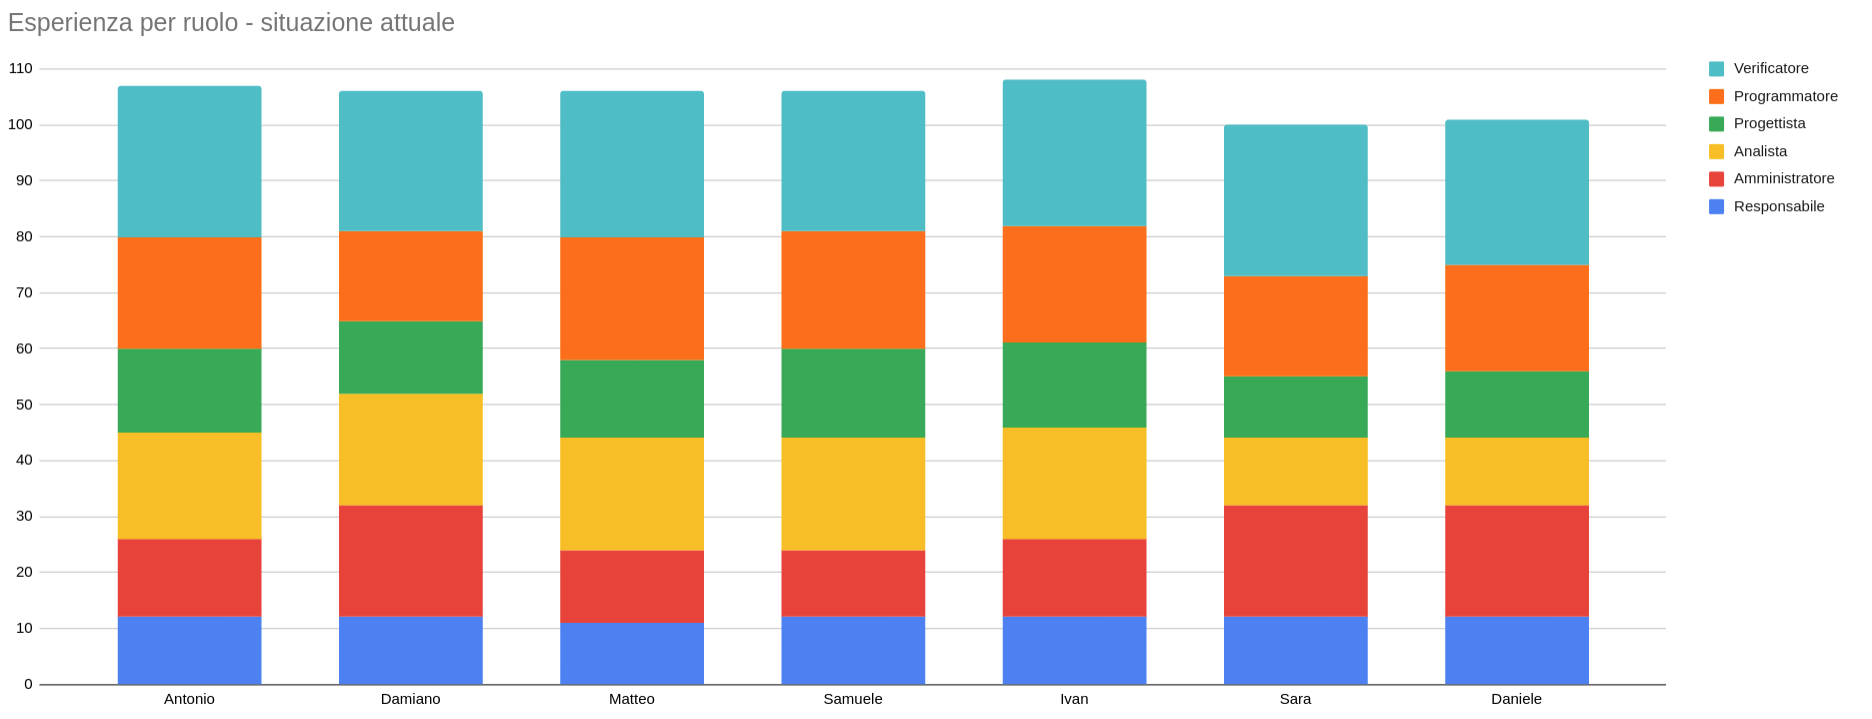
\includegraphics[width=15cm]{res/images/GraficoRuoliDettaglioCodifica.png}
	\caption*{\textbf{Figura 15}: Esperienza per ruolo}
	\label{fig:Esperienza per ruolo}
\end{figure}

\subsubsection{Consuntivo di microperiodo}
\paragraph{Microperiodo 1}
\begin{table}[H]
	\rowcolors{2}{lightest-grayest}{white}
	\centering
	\begin{tabular}{|c|c|c|c|c|c|c|}
		\hline
		\rowcolor{lighter-grayer}
		\textbf{Attività} & \textbf{Re}        & \textbf{Am}        & \textbf{An}        & \textbf{Pt}        & \textbf{Pm}        & \textbf{Ve}        \\ \hline
		
		Comunicazione con proponente & 1 & - & - & - & - & - \\ \hline
		PoC mobile & 2 & - & - & 16 & 16 & - \\ \hline
		Configurazione analisi statica, CI, etc.. & 3 & - & - & 7 & - & - \\ \hline
		
	\end{tabular}
	\caption*{\textbf{Tabella 24}: Prospetto orario reale\\}
\end{table}

\begin{table}[H]
	\rowcolors{2}{lightest-grayest}{white}
	\centering
	\renewcommand{\arraystretch}{1.5}
	\begin{tabular}{|c|c|c|}
		\hline
		\rowcolor{lighter-grayer}
		Ruolo & Ore & Costo \\ \hline
		Responsabile & 6(+0) & 180(+0\euro) \\ \hline
		Amministratore & - & - \\ \hline
		Analista & - & - \\ \hline
		Progettista & 16(+0) & 384(+0\euro) \\ \hline
		Programmatore & 23(+4) & 368(+64\euro) \\ \hline
		Verificatore & - & - \\ \hline
		Totale preventivo & 41 & 868\euro \\ \hline
		Totale consuntivo & 45 & 932\euro \\ \hline
		Totale scostamento & 4 & 64\euro \\ \hline
	\end{tabular}
	\caption*{\textbf{Tabella 25}: Consuntivo\\}
\end{table}

\paragraph{Microperiodo 2}
\begin{table}[H]
	\centering
	\begin{tabular}{|c|c|c|c|c|c|c|}
		\hline
		\rowcolor{lighter-grayer}
		\textbf{Attività} & \textbf{Re}        & \textbf{Am}        & \textbf{An}        & \textbf{Pt}        & \textbf{Pm}        & \textbf{Ve}        \\ \hline
		
		Aggiornamento AdR & 1 & - & 12 & - & - & 2 \\ \hline
		Aggiornamento PdQ & 1 & - & - & - & - & 6 \\ \hline
		Aggiornamento PdP & 4 & - & - & - & - & 1 \\ \hline
		Aggiornamento NdP & 1 & 1 & - & - & - & 1 \\ \hline
		Comunicazione con docenti & 1 & - & - & - & - & - \\ \hline
		
	\end{tabular}
	\caption*{\textbf{Tabella 24}: Prospetto orario reale\\}
\end{table}

\begin{table}[H]
	\rowcolors{2}{lightest-grayest}{white}
	\centering
	\renewcommand{\arraystretch}{1.5}
	\begin{tabular}{|c|c|c|}
		\hline
		\rowcolor{lighter-grayer}
		Ruolo & Ore & Costo \\ \hline
		Responsabile & 8(+0) & 240(+0\euro) \\ \hline
		Amministratore & 1(+0) & 22(+0\euro) \\ \hline
		Analista & 12(+0) & 300(+0\euro) \\ \hline
		Progettista & - & - \\ \hline
		Programmatore & - & - \\ \hline
		Verificatore & 10(-1) & 160(-16\euro) \\ \hline
		Totale preventivo & 32 & 738\euro \\ \hline
		Totale consuntivo & 31 & 722\euro \\ \hline
		Totale scostamento & 1 & 16\euro \\ \hline
	\end{tabular}
	\caption*{\textbf{Tabella 25}: Consuntivo\\}
\end{table}

\paragraph{Microperiodo 3}
\begin{table}[H]
	\centering
	\begin{tabular}{|c|c|c|c|c|c|c|}
		\hline
		\rowcolor{lighter-grayer}
		\textbf{Attività} & \textbf{Re}        & \textbf{Am}        & \textbf{An}        & \textbf{Pt}        & \textbf{Pm}        & \textbf{Ve}        \\ \hline
		
		Configurazione del sistema & 1 & - & - & - & 6 & 2 \\ \hline
		Comunicazione con docenti & 1 & - & - & - & - & - \\ \hline	
		
	\end{tabular}
	\caption*{\textbf{Tabella 24}: Prospetto orario reale\\}
\end{table}

\begin{table}[H]
	\rowcolors{2}{lightest-grayest}{white}
	\centering
	\renewcommand{\arraystretch}{1.5}
	\begin{tabular}{|c|c|c|}
		\hline
		\rowcolor{lighter-grayer}
		Ruolo & Ore & Costo \\ \hline
		Responsabile & 2(+0) & 60(+0\euro) \\ \hline
		Amministratore & - & - \\ \hline
		Analista & - & - \\ \hline
		Progettista & - & - \\ \hline
		Programmatore & 6(+1) & 96(+16\euro) \\ \hline
		Verificatore & 2(+0) & 32(+0\euro) \\ \hline
		Totale preventivo & 9 & 172\euro \\ \hline
		Totale consuntivo & 10 & 188\euro \\ \hline
		Totale scostamento & 1 & 16\euro \\ \hline
	\end{tabular}
	\caption*{\textbf{Tabella 25}: Consuntivo\\}
\end{table}

\paragraph{Microperiodo 4}
\begin{table}[H]
	\centering
	\begin{tabular}{|c|c|c|c|c|c|c|}
		\hline
		\rowcolor{lighter-grayer}
		
		\textbf{Attività}                         & \textbf{Re} & \textbf{Am} & \textbf{An} & \textbf{Pt} & \textbf{Pm} & \textbf{Ve} \\ \hline
		PB                                        & 1           & -           & -           & 14          & -           & 2           \\ \hline
		Codifica della struttura delle componenti & 1           & -           & -           & -           & 15          & 7           \\ \hline	
		
	\end{tabular}
	\caption*{\textbf{Tabella 24}: Prospetto orario reale\\}
\end{table}

\begin{table}[H]
	\rowcolors{2}{lightest-grayest}{white}
	\centering
	\renewcommand{\arraystretch}{1.5}
	\begin{tabular}{|c|c|c|}
		\hline
		\rowcolor{lighter-grayer}
		Ruolo & Ore & Costo \\ \hline
		Responsabile & 2(+0) & 60(+0\euro) \\ \hline
		Amministratore & - & - \\ \hline
		Analista & - & - \\ \hline
		Progettista & 14(+0) & 336(+0\euro) \\ \hline
		Programmatore & 15(+0) & 240(+0\euro) \\ \hline
		Verificatore & 9(+0) & 144(+0\euro) \\ \hline
		Totale preventivo & 40 & 780\euro \\ \hline
		Totale consuntivo & 40 & 780\euro \\ \hline
		Totale scostamento & - & - \\ \hline
	\end{tabular}
	\caption*{\textbf{Tabella 25}: Consuntivo\\}
\end{table}

\paragraph{Microperiodo 5}
\begin{table}[H]
	\centering
	\begin{tabular}{|c|c|c|c|c|c|c|}
		\hline
		\rowcolor{lighter-grayer}
		\textbf{Attività} & \textbf{Re}        & \textbf{Am}        & \textbf{An}        & \textbf{Pt}        & \textbf{Pm}        & \textbf{Ve}        \\ \hline
		
		Aggiornamento AdR                         & 1 & - & 8 & - & -  & 1 \\ \hline
		PB                                        & 1 & - & - & 5 & -  & 2 \\ \hline
		Codifica della struttura delle componenti & 1 & - & - & - & 20 & 8 \\ \hline		
		
	\end{tabular}
	\caption*{\textbf{Tabella 24}: Prospetto orario reale\\}
\end{table}

\begin{table}[H]
	\rowcolors{2}{lightest-grayest}{white}
	\centering
	\renewcommand{\arraystretch}{1.5}
	\begin{tabular}{|c|c|c|}
		\hline
		\rowcolor{lighter-grayer}
		Ruolo & Ore & Costo \\ \hline
		Responsabile & 3(+0) & 90(+0\euro) \\ \hline
		Amministratore & - & - \\ \hline
		Analista & 8(+0) & 200(+0\euro) \\ \hline
		Progettista & 5(+0) & 120(+0\euro) \\ \hline
		Programmatore & 20(+0) & 320(+0\euro) \\ \hline
		Verificatore & 11(+0) & 176(+0\euro) \\ \hline
		Totale preventivo & 47 & 906\euro \\ \hline
		Totale consuntivo & 47 & 906\euro \\ \hline
		Totale scostamento & - & - \\ \hline
	\end{tabular}
	\caption*{\textbf{Tabella 25}: Consuntivo\\}
\end{table}

\paragraph{Microperiodo 6}
\begin{table}[H]
	\centering
	\begin{tabular}{|c|c|c|c|c|c|c|}
		\hline
		\rowcolor{lighter-grayer}
		\textbf{Attività} & \textbf{Re}        & \textbf{Am}        & \textbf{An}        & \textbf{Pt}        & \textbf{Pm}        & \textbf{Ve}        \\ \hline
		
		Codifica delle interazioni tra le componenti interne & 2           & -           & -           & -           & 35          & 15          \\ \hline
		Codifica delle interazioni con gli attori esterni    & 1           & -           & -           & -           & 15          & 6           \\ \hline
		
	\end{tabular}
	\caption*{\textbf{Tabella 24}: Prospetto orario reale\\}
\end{table}

\begin{table}[H]
	\rowcolors{2}{lightest-grayest}{white}
	\centering
	\renewcommand{\arraystretch}{1.5}
	\begin{tabular}{|c|c|c|}
		\hline
		\rowcolor{lighter-grayer}
		Ruolo & Ore & Costo \\ \hline
		Responsabile & 3(+0) & 90(+0\euro) \\ \hline
		Amministratore & - & - \\ \hline
		Analista & - & - \\ \hline
		Progettista & - & - \\ \hline
		Programmatore & 50(+0) & 800(+0\euro) \\ \hline
		Verificatore & 21(+0) & 336(+0\euro) \\ \hline
		Totale preventivo & 74 & 1226\euro \\ \hline
		Totale consuntivo & 74 & 1226\euro \\ \hline
		Totale scostamento & - & - \\ \hline
	\end{tabular}
	\caption*{\textbf{Tabella 25}: Consuntivo\\}
\end{table}

\paragraph{Microperiodo 7}
\begin{table}[H]
	\centering
	\begin{tabular}{|c|c|c|c|c|c|c|}
		\hline
		\rowcolor{lighter-grayer}
		\textbf{Attività} & \textbf{Re}        & \textbf{Am}        & \textbf{An}        & \textbf{Pt}        & \textbf{Pm}        & \textbf{Ve}        \\ \hline
		
		Aggiornamento PdQ   & 1 & -  & - & - & - & 8 \\ \hline
		Aggiornamento PdP   & 6 & -  & - & - & - & 1 \\ \hline
		Codifica delle interazioni con gli attori esterni & 1           & -           & -           & -           & 20          & 8           \\ \hline
		Manuale utente      & 1 & 12 & - & - & - & 4 \\ \hline
		Manuale manutentore &   & 12 & - & - & - & 4 \\ \hline
	
	\end{tabular}
	\caption*{\textbf{Tabella 24}: Prospetto orario reale\\}
\end{table}

\begin{table}[H]
	\rowcolors{2}{lightest-grayest}{white}
	\centering
	\renewcommand{\arraystretch}{1.5}
	\begin{tabular}{|c|c|c|}
		\hline
		\rowcolor{lighter-grayer}
		Ruolo & Ore & Costo \\ \hline
		Responsabile & 9(+0) & 270(+0\euro) \\ \hline
		Amministratore & 24(+0) & 528(+0\euro) \\ \hline
		Analista & - & - \\ \hline
		Progettista & - & - \\ \hline
		Programmatore & 20(+0) & 320(+0\euro) \\ \hline
		Verificatore & 25(+0) & 400(+0\euro) \\ \hline
		Totale preventivo & 78 & 1518\euro \\ \hline
		Totale consuntivo & 78 & 1518\euro \\ \hline
		Totale scostamento & - & - \\ \hline
	\end{tabular}
	\caption*{\textbf{Tabella 25}: Consuntivo\\}
\end{table}

\paragraph{Altro}
\begin{table}[H]
	\centering
	\begin{tabular}{|c|c|c|c|c|c|c|}
		\hline
		\rowcolor{lighter-grayer}
		\textbf{Attività} & \textbf{Re}        & \textbf{Am}        & \textbf{An}        & \textbf{Pt}        & \textbf{Pm}        & \textbf{Ve}        \\ \hline
		
		Presentazione       & 1           & 1           & 1           & 1           & 1           & 1           \\ \hline
		Attività accessorie & 2           & 5           & 1           & 1           & 2           & 3           \\ \hline
		
	\end{tabular}
	\caption*{\textbf{Tabella 24}: Prospetto orario reale\\}
\end{table}

\begin{table}[H]
	\rowcolors{2}{lightest-grayest}{white}
	\centering
	\renewcommand{\arraystretch}{1.5}
	\begin{tabular}{|c|c|c|}
		\hline
		\rowcolor{lighter-grayer}
		Ruolo & Ore & Costo \\ \hline
		Responsabile & 3(+0) & 90(+0\euro) \\ \hline
		Amministratore & 6(+0) & 132(+0\euro) \\ \hline
		Analista & 2(+0) & 50(+0\euro) \\ \hline
		Progettista & 2(+0) & 48(+0\euro) \\ \hline
		Programmatore & 3(+0) & 48(+0\euro) \\ \hline
		Verificatore & 4(+0) & 64(+0\euro) \\ \hline
		Totale preventivo & 20 & 432\euro \\ \hline
		Totale consuntivo & 20 & 432\euro \\ \hline
		Totale scostamento & - & - \\ \hline
	\end{tabular}
	\caption*{\textbf{Tabella 25}: Consuntivo\\}
\end{table}

\subsubsection{Preventivo a finire}
